%!TEX root = ../main.tex
\section{Three phase inverter}
\label{sec:inverter}
This section will describe the design of the three-phase inverter used to drive the PMAC motor in this project.
This includes the calculations and considerations done.
Initially, a short overview of the principle of operation of a three-phase inverter is given.

\subsection{Principle of Operation of the Three-Phase Inverter}
\todo[inline]{Thomas: I have to question whether this is the appropriate title for this section?}
A three-phase inverter enables the use of a DC supply in variable frequency control of a three-phase load.
In this project the DC supply is a battery and the load, a PMAC motor.
Figure \ref{fig:threephaseinverter} is a simulink model showing the most basic three-phase inverter.
As can be seen, the inverter consists of three half-bridges for a total of six switches.
Each pair of switches can never be on at the same time as this would result in shorting the battery.

\begin{figure}[!h]
	\centering
	\includegraphics[width=\linewidth,trim=0cm 5cm 0cm 1cm]{graphics/threephaseinverter}
	\caption{Simulink model of a simple three-phase inverter for a balanced load.}
	\label{fig:threephaseinverter}
\end{figure}

This type of inverter only works with a balanced load, such as the PMAC motor.
A balanced three-phase load implies, that the sum of current in the three phases is zero, and no current through a neutral wire.
As the inverter does not have a connection to the neutral point of the load, it could not supply an unbalanced load, such as those in UPS'es and solar cells.
\todo[inline]{Martin: added something about it being a balanced load}

Several schemes exist to control the switches.
Throughout this project a PWM modulation technique using sinusoids as reference is used.
Figure \ref{fig:countercarrier} is a depiction of the modulation technique.
A counter is continuously counting up and down, creating a triangle wave.
\todo[inline]{Martin: This is not about the software, so how we generate the PWM isn necessary}
This is called the carrier wave.
The carrier wave is compared to a sinusoidal reference signal.
The frequency of the sinusoidal will be the fundamental frequency of the output voltage.
\todo[inline]{Martin: Not sure what you mean by output voltage}
Whenever the reference cross the carrier wave, the gate voltages of the relevant half-bridge invert, of course taking into account the necessary dead time to avoid short circuiting the power rail.
This technique produces naturally sampled PWM, a desirable trait due to the lower harmonic distortion when compared to other types of PWM.
Additionally, the speed of the motor can be easily changed simply by changing the fundamental frequency.

\begin{figure}[h!]
	\centering
	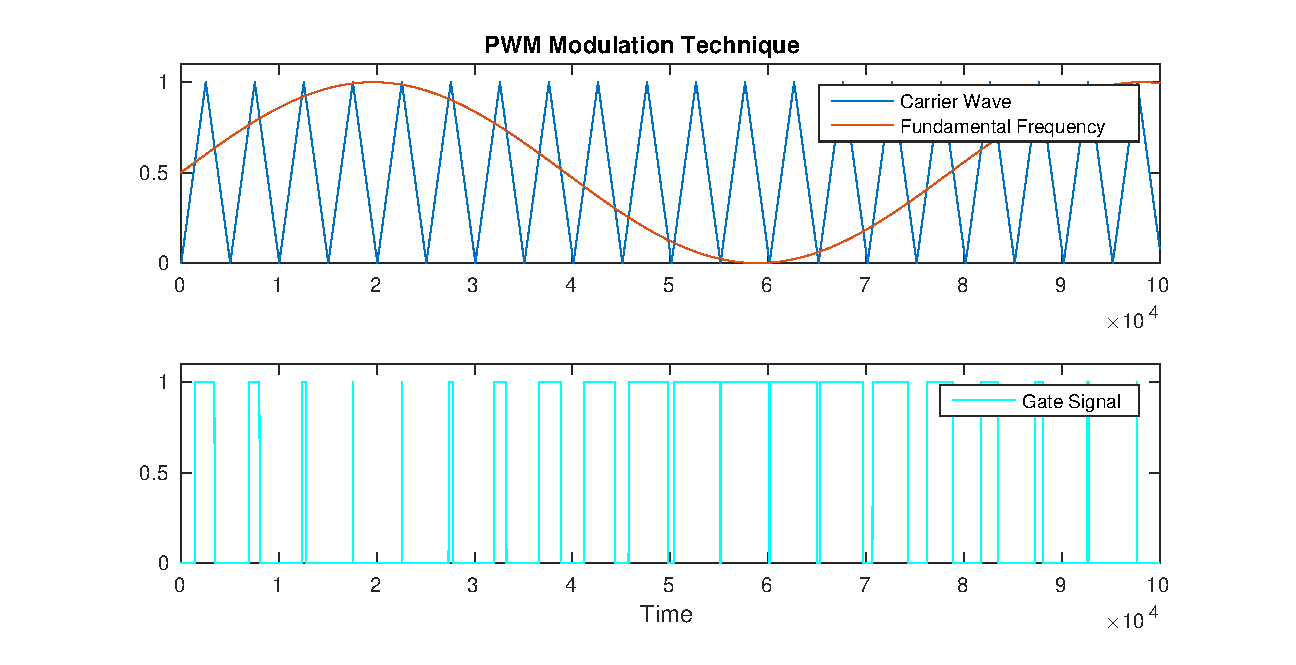
\includegraphics[width=\linewidth]{graphics/countercarrier}
	\caption{Naturally sampled PWM using a sinusoid as fundamental frequency.}
	\label{fig:countercarrier}
\end{figure}
\todo[inline]{Martin: Maybe get a darker color for the lower plot}
\todo[inline]{Martin: We should extend this to a three phase inverter, as this is only one half bridge, and that is not even a DC inverter}

\subsection{Choosing the MOSFETs}\label{sub:choosing_mosfets}
\label{sec:mosfet}
Before choosing MOSFETs for the three phase inverter one will have to keep in mind the application parameters.
Firstly the batteries\cite{superB} will have average nominal voltage of $52.8V$ and end of charge voltage at $60.8V$.
The MOSFETs will therefor need to be able to handle a minimum drain to source voltage, $V_{DS}$, of 60.8V. 
Secondly, the current drawn by the motor can reach a maximum peak of 300A.
Thirdly, the motor driver\cite{DRV8301} will supply a gate voltage, $V_{GS}$, of 9.5V to 11.5V. 
The MOSFETs will therefor need to be fully conducting at $V_{GS} = 9.5V$ and be able to handle the driver supplied range.
The three main requirements are listed in table \ref{tab:req1}\\

\begin{table}[h!]
	\caption{Three main requirements as a starting point for choosing the MOSFETs}
	\centering
	\begin{tabular}{clr}
		  & Requirement\\
		  \hline
		1 & Can handle minimum voltage of & 60.8V\\
		2 & Can handle minimum current of & 300A\\
		3 & Operating at $V_{GS}$ of  & 9.5V \\
		\hline
	\end{tabular}
	\label{tab:req1}
\end{table}

Due to high currents through the MOSFETs, the heat dissipation is assumed to be high as well. 
To prevent overheating and burning out the MOSFETs they will be mounted on to a heat sink. 
Therefore a through hole package will be required for this application. 
Because of its size and easy mounting, the chosen package is the TO-247 package\cite{TO_247}. When looking for MOSFETs that add up to the requirements of table~\ref{tab:req1}, the International rectifier power MOSFET IRFP4468PBF is chosen.

\begin{table}[h!]
	\centering
	\caption{Some important parameters from the IRFP4468PBF MOSFET datasheet\cite{IRF4468PbF}. All parameters are found at junction temperature $T_J = 25^{\circ}$C}
\begin{tabular}{|l|l|c|c|c|c|}
	\hline
	\multicolumn{1}{|c|}{Symbol} & \multicolumn{1}{|c|}{Parameter} & Min. & Typ. &
	 Max. & Units\\
	\hline
	$I_D$ & Continuous Drain Current (Silicon Limited) & - & - & 290 & A\\
	\hline
	$I_D$ & Continuous Drain Current (Package Limited) & - & - & 195 & A\\
	\hline
	$V_{GS}$ & Gate to Source Voltage & - & - & $\pm$20 & V\\
	\hline
	 $V_{GS(th)}$ & Gate Threshold Voltage & 2.0 & - & 4.0 & V\\
	 \hline
	 $V_{(BR}DSS$ & Drain to Source Breakdown Voltage & 100 & - & - & V\\
	 \hline
	 $R_{DS(on)}$ & Static Drain to Source On Resistance & - & 2.0 & 2.6 & m$\Omega$\\
	 \hline
	 
\end{tabular}
\label{tab:MOSdata}
\end{table}
The TO-247 package has a continuous drain current limit of 195A that is only around two third of the minimum current requirement. 
With that in mind, the MOSFET parameters in table~\ref{tab:MOSdata} seem to be a  suitable chose for the application if more than one MOSFET is used for each switching side. 
Using the parallel setup, the MOSFETs are assumed to share the current equally. 
If one would draw more current than the others, the temperature would rise causing $R_{DS(on)}$ to rise as seen in figure~\ref{fig:tj_rds}. 
That will then result in reduced current.
As will be later discussed, parallel setup will also have effect on the total power loss.


\subsection{Power Loss}

The total power loss, $P_{loss}$ of a switching device can be estimated using equation~\ref{eq:p_loss} where $P_c$ and $P_{sw}$ are conduction- and switching losses respectively.  

\begin{equation}
P_{loss} = P_{c} + P_{sw}
\label{eq:p_loss}
\end{equation}

For simplicity the power loss will be estimated from a single phase of the inverter circuit seen in figure~\ref{fig:single_phase}. 
The current $I_{out}$ is drawn by some load $R_{load}$ that will absorb the load power $P_{load}$ which is given by equation\ref{eq:p_load}. 
Since there are two switches, $Q_1$ and $Q_2$, it is assumed that the load power is delivered equally from both. The output power, $P_{Q}$, of each switch is given by equation~\ref{eq:P_Q}  


\begin{figure}[!h]
	\centering
	\includestandalone[width=0.2\textwidth]{graphics/mosfets}
	\caption{Single phase}
	\label{fig:single_phase}
\end{figure}


\begin{equation}
P_{load} = R_{load} I_{out,rms}^2
\label{eq:p_load}
\end{equation}

\begin{equation}
P_{Q} = \dfrac{P_{load}}{2} = R_{load} I_{Qi,rms}^2
\label{eq:P_Q}
\end{equation}


With insertion of equation~\ref{eq:p_load} into~\ref{eq:P_Q} and solving for $I_{Qi,rms}$, equation~\ref{eq:I_qrms} is formed.

\begin{equation}
\dfrac{R_{load} I_{out,rms}^2}{2} = R_{load} I_{Qi,rms}^2 \rightarrow I_{Qi,rms} = \dfrac{I_{out,rms}}{\sqrt{2}} 
\label{eq:I_qrms}
\end{equation}
Which then again can be expressed as in equation~\ref{eq:I_qi}.

\begin{equation}
I_{Qi,rms} = \dfrac{I_{out,rms}}{\sqrt{2}} = \dfrac{I_{out}}{\sqrt{2}\sqrt{2}} = \dfrac{I_{out}}{2}
\label{eq:I_qi}
\end{equation}


As mentioned earlier each switching setup will consist of $n$ number of MOSFETs in parallel. Therefor the Drain current of each parallel MOSFET becomes $I_{Pi,rms}$ in equation~\ref{eq:I_pi}.

\begin{equation}
I_{Pi,rms}=\dfrac{I_{Qi,rms}}{n} = \dfrac{I_{out}}{2n}
\label{eq:I_pi}
\end{equation}

\subsubsection{Conduction loss}\label{sub:Cunduction_loss}


Conduction loss of the MOSFETs can be calculated using equation~\ref{eq:p_c}

\begin{equation}
P_{c} = R_{DS(on)} I_{Pi,rms}^2
\label{eq:p_c}
\end{equation}


Although listed in the datasheet, the drain to source resistance $R_{DS(on)}$ only applies to the  $T_J = 25 \si{\celsius}$ condition. 
The resistance will vary with the junction temperature $T_J$. 
The relation between $T_J$ and $R_{DS(on)}$ can be seen in figure~\ref{fig:tj_rds} from where the multiplication factor $\alpha$ in equation~\ref{eq:Rdstj} can be estimated.

\begin{equation}
R_{DS(on),@T_J} =  \alpha R_{DS(on),@25\si{\celsius}}
\label{eq:Rdstj}
\end{equation}

\begin{figure}[h!]
	\centering
	\includegraphics[scale =0.7]{graphics/T_n_R_compare}
	\caption{The $R_{DS(on)}$ and $T_J$ relation at $I_D = 180A$ and $V_{GS} = 10V$}
	\label{fig:tj_rds}
\end{figure}

If assumed that the junction temperature will be around $100 \si{\celsius}$ one can estimate the factor being somewhere close to $\alpha = 1.6$. 
The instantaneous conduction loss for each MOSFET in parallel can then be estimated using equations~\ref{eq:p_c}, \ref{eq:I_pi} and \ref{eq:Rdstj} to form equation~\ref{eq:P_cp}.

\begin{equation}
P_{c} = R_{DS(on),@100\si{\celsius}} I_{Pi,rms}^2 =  R_{DS(on),@100\si{\celsius}} \bigg(\dfrac{I_{out}}{2n}\bigg)^2
\label{eq:P_cp}
\end{equation}

\subsubsection{Switching loss}
Whenever any MOSFET is switching from its on state to its off state or vice versa, a small amount of energy is lost, as the MOSFET passes through its active region.
This loss can be found with experiments or estimated from calculations. 
An experiment will not be carried out at this point but the loss will be estimated with calculations and assumptions using equation~\ref{eq:P_sw}.

\begin{equation}
P_{sw} = \dfrac{1}{2} V_{in} I_D (t_{c,on} + t_{c,off} ) f_{s}
\label{eq:P_sw}
\end{equation}

where $I_D$ is the drain current, $I_{Pi,rms}$, of each MOSFET from equation~\ref{eq:I_pi} and $\mathrm{V_{in}}$ is the supply voltage for the inverter. 
The times $t_{c,on} $ and $ t_{c,off} $ are the combined on and off time respectively and are defined in figure~\ref{fig:sw_loss} as equation~\ref{eq:time_on} and~\ref{eq:time_off}

\begin{figure}[h!]
	\centering
	\includegraphics[scale = 0.5]{graphics/sw_losses}
	\caption[MOSFET switching losses.]{MOSFET switching losses. $t_{ri}$ and $t_{fi}$ are the current,$I_D$, rise and fall times respectively and $t_{rv}$ and $t_{fv}$ are the rise and fall time of $D_{DS}$ respectively.}
	\label{fig:sw_loss}
\end{figure}

\begin{eqnarray}
t_{c,on} = t_{ri} + t_{fv}
\label{eq:time_on}\\
t_{c,off} = t_{rv} + t_{fi}
\label{eq:time_off}
\end{eqnarray}

The voltage rise and fall times $t_{rv}$ and $t_{fv}$ respectively in figure~\ref{fig:sw_loss} are the time it takes the drain to source voltage, $V_{DS}$ to rise from zero to $V{in}$ and opposite. 
The values are defined in the MOSFET datasheet\cite{IRF4468PbF} as the rise and fall times $t_r$ and $t_f$ seen in figure~\ref{fig:sw_time_wavef}. 
The times are listed in table~\ref{tab:tf_tr}.
Equation~\ref{eq:tfv_tr} and \ref{eq:trv_tf} show the relation.

\begin{figure}[h!]
	\centering
	\includegraphics[scale = 0.5]{graphics/sw_time_wavef}
	\caption{Switching Time Waveforms where }
	\label{fig:sw_time_wavef}
\end{figure}

\begin{table}[h!]
	\centering
	\caption{$V_{GS}$ rise and fall time taken from datasheet}
	\begin{tabular}{|c|c|c|c|}
		\hline
		Symbol & Parameter & Typ. & Units\\
		\hline
		$t_r$ & Rise Time & 230 & ns\\
		$t_f$ & Fall Time & 260 & ns\\
		\hline
	\end{tabular}
	\label{tab:tf_tr}
\end{table}


\begin{eqnarray}
t_{fv} = t_r\label{eq:tfv_tr}\\
t_{rv} = t_f\label{eq:trv_tf}
\end{eqnarray}

The turn on and off characteristics of the MOSFETs are shown in figure~\ref{fig:turn_on_off}. 
From there one can see that the current rise and fall times, $t_{ri}$ and $t_{fi}$ respectively, are the same times as it takes the gate voltage $V_{GS}$ to rise from $V_{GS(th)}$ to $V_{GS(I_0)}$ for the on state and opposite for the off state.



\begin{figure}[h!]
	\centering
	\begin{subfigure}[b]{0.4\textwidth}
		\includegraphics[width=\textwidth]{graphics/mos_turn_on}
		\caption{turn on}
		\label{fig:Turn_on}
	\end{subfigure}
	~
	\begin{subfigure}[b]{0.4\textwidth}
		\includegraphics[width=\textwidth]{graphics/mos_turn_off}
		\caption{turn off}
		\label{fig:Turn_off}
	\end{subfigure}
	\caption{the turn on and off characteristics of the MOSFETs.}
	\label{fig:turn_on_off}
\end{figure}

The gate to source current, $I_(gs)$ is defined in equation\ref{eq:I_gs} where $dt$ are the current rise and fall times $t_{ri}$ and $t_{fi}$ respectively. 
$dV$ is the difference between $V_{GS(th)}$ and $V_{GS(I_0)}$ as seen in equation~\ref{eq:dv} and n is the number of MOSFETs in parallel.

\begin{equation}
I_{gs} = nC\dfrac{dV}{dt} 
\label{eq:I_gs}
\end{equation}

\begin{equation}
dV = |V_{GS(I_0)} - V_{GS(th)}|
\label{eq:dv}
\end{equation}

For simplicity it is assumed that the gate charge current remains constant. 
Then one can assume that the gate to source current is known. 
The motor driver sources up to $1.7A$ when in the on state and sinks up to $2A$ when in off state\cite{DRV8301}. 
Equation~\ref{eq:I_gs} can then be rearranged for $dt$ as shown in equation~\ref{eq:dt}. 
It is assumed that the charge current will be a constant for.

\begin{equation}
dt = nC\dfrac{dV}{I_{gs}}
\label{eq:dt}
\end{equation}



\subsection{Total Power loss}

The instantaneous power losses are calculated for up to 10 MOSFETs in parallel using equations~\ref{eq:P_cp}, \ref{eq:P_sw} and~\ref{eq:p_loss} where the switching frequency is $f_s = 20kHz$. Figures~\ref{fig:ploss_single} and~\ref{fig:ploss_comb} show the results.


\begin{figure}[h!]
	\centering
	\includegraphics[scale = 0.5]{graphics/pwr_loss_single}
	\caption{Instantaneous Power losses of a single MOSFET in a parallel setup as a function of number of MOSFETs}
	\label{fig:ploss_single}
\end{figure}

In Figure~\ref{fig:ploss_single} the losses are calculated for each MOSFET in a parallel setup of $n$ MOSFETs. 
One will notice, as former stated, that the number of MOSFETs in parallel, effects the power loss much.
The conduction loss will decrease fast and will become close to nothing when $n$ increases. 
This happens because the current is equally divided between the MOSFETs, thus, each MOSFET has less current flowing through. 
The switching loss however increases with $n$ and will become dominant. In that case the gate capacitance will increase by a factor of $n$ causing the switching loss to increase.

\begin{figure}[h!]
	\centering
	\includegraphics[scale = 0.5]{graphics/pwr_loss_comb}
	\caption{Combined instantaneous power losses of each parallel setup as a function of number of MOSFETs}
	\label{fig:ploss_comb}
\end{figure}

From the combined power loss shown in figure~\ref{fig:ploss_comb}, it is clear that the total instantaneous power loss is smallest when $n = 2$ or $P_{loss} \approx 95W$. 
The design will have two MOSFETs in parallel switching each phase. The total instantaneous power loss will then become for all three phases as seen in equation~\ref{eq:P_loss_total}.
\begin{equation}
P_{loss,total} = 95*6 = 570W
\label{eq:P_loss_total}
\end{equation}

\subsection{Temperature}

The power losses defined in previous sections will cause the MOSFETs to heat up while operating. 
Therefore they will be mounted on to a heat sink as mentioned in section\ref{sub:choosing_mosfets}. 
To get an estimate on how hot the MOSFETs will be, equations~\ref{eq:Ta}, \ref{eq:Tc} and \ref{eq:Tj} are used. 
$T_s$ is the MOSFET source temperature, $T_c$ the case temperature  and $T_j$ is the junction temperature.
The parameter can be seen in table~\ref{tab:temp_param}. 
to get some idea of the temperature it is assumed that the time it takes the motor to get from zero to full power, $t = 5s$. 
The system will for that time be operating at maximum torque.
in reality, other factors will effect the power dissipation but will not be discussed further.
 

\begin{table}[h!]
	\centering
	\caption{Parameters used to calculate the temperature}
	\begin{tabular}{|c|l|c|c|}
		\hline
		Symbol & \multicolumn{1}{c|}{Parameter} & Value & Units\\
		\hline
		$T_{J,max}$ & MOSFET maximum junction temperature & 175 & \si{\celsius}\\
		\hline
		$R_{jc}$ & MOSFET Junction to Case thermal resistance & 0.29 & \multirow{3}{*}{\si{\celsius/W}}\\
		\cline{1-3}
		$Re_{cs}$ & MOSFET Case to Sink thermal resistance & 0.24 &\\
		\cline{1-3}
		$R_{sa}$ & heat sink Thermal resistance & 0.29 & \\
		\hline
		$C_s$ & heat sink Thermal capacitance  & 2190 &\si{\joule/\celsius}\\
		\hline
		$P_{loss,total}$ & instantaneous power loss of each MOSFET & 570 & \si{\watt}\\
		\hline
	\end{tabular}
	\label{tab:temp_param}
\end{table}



\begin{eqnarray}
T_s  & = & (R_{sa}P_{loss,total})\bigg(1-exp(-\dfrac{t}{R_{sa}C_s})\bigg) + T_a
\label{eq:Ta}\\
T_c & = & T_s + P_{loss}R_{cs}
\label{eq:Tc}\\
T_j & = & T_c + P_{loss}R_{jc}
\label{eq:Tj}
\end{eqnarray}


The temperatures are calculated to be:

\begin{eqnarray*}
T_s & = &  26\si{\celsius}\\
T_c & = &  49\si{\celsius}\\
T_j & = &  77\si{\celsius}\\
\end{eqnarray*}

The calculated junction temperature is well below the maximum ratings shown in table~\ref{tab:temp_param}. It is safe to assume that the MOSFETs will not reach the maximum.